\section{Series de potencias. Series de Fourier. Ecuaciones diferenciales}
\subsection{Introducción}
Sea $(f_n)_n$ una sucesión de funciones reales definidas todas en un mismo intervalo $I$ de la recta real. Para cada punto $x\in I$ tendremos una sucesión de números reales $(f_n(x))_n$ y también podemos considerar la serie numérica $\sum f_n(x)$ correspondiente. Supongamos que esta serie es convergente para todos los puntos $x$ de un cierto subconjunto de $M$ del intervalo $I$. Haciendo corresponder a cada $x\in M$ el valor $S(x)$ de la suma de la serie $\sum f_n(x)$, tendremos definida una nueva función en el conjunto $M$, que llamaremos función suma de la serie de funciones $\sum f_n$. El conjunto $M$ de todos los puntos en los cuales la serie es convergente se llama campo de convergencia de la serie funcional $\sum f_n$.
\begin{itemize}[label=\color{red}\textbullet, leftmargin=*]
	\item \color{lightblue}Ejemplo
\end{itemize}
Consideremos la sucesión de funciones $(f_n)_n$ dada por $f_n(x)=x^n$. Para cada $x\in\mathbb{R}$ la serie numérica $\sum x^n$ es una serie geométrica de razón $x$. Si $|x|<1$, la serie es convergente, luego el intervalo $(-1,1)$ está contenido en el campo de convergencia de la serie $\sum f_n$. Si $|x|>1$, la serie es divergente. Para $x=1$ y $x=-1$ las series son divergente y no sumable respectivamente. Luego el campo de convergencia es el intervalo abierto $(-1,1)$.
\subsection{Convergencia puntual}
\begin{itemize}[label=\color{red}\textbullet, leftmargin=*]
	\item \color{lightblue}Definición
\end{itemize}
Sea $I$ un subconjunto de $\mathbb{R}$. Supongamos que para cada número natural $n$ está dada una función $f_n:I\rightarrow\mathbb{R}$; la aplicación $n\rightarrow f_n$ recibe el nombre de sucesión de funciones. La función $f_n$ asociada al número natural $n$ recibe el nombre de término $n$-ésimo de la sucesión.

Informalmente, una sucesión de funciones es una lista sin fin \[ f ,~f_2,~\hdots,~f_n,~\hdots \] de funciones definidas en el punto $I$. Para cada punto $x\in I$ podemos considerar la sucesión de números reales que tiene por término $n$-ésimo real $f_n(x)$, valor en $x$ de la función $f_n$. Esta sucesión podrá ser convergente o no.
\begin{itemize}[label=\color{red}\textbullet, leftmargin=*]
	\item \color{lightblue}Definición
\end{itemize}
Sea $(f_n)_n$ una sucesión de funciones definidas en el conjunto $I,M$ un subconjunto de $I$ y $f$ una función definida en $M$. Si para cada $x\in M,f(x)=\lim_{n\to\infty}f_n(x)$, se dice que la sucesión $(f_n)_n$ convergente puntualmente a $f$ en $M$, o que converge punto a punto a $f$ en $M$. Cuando existe tal función $f$, decimos que la sucesión $(f_n)_n$ es convergente punto a punto en $M$, o que la sucesión $(f_n)$ es convergente puntualmente en $M$.
\begin{itemize}[label=\color{red}\textbullet, leftmargin=*]
	\item \color{lightblue}Ejemplo
\end{itemize}
La sucesión $(x^n)_n$ converge puntualmente en el intervalo cerrado $ [0,1]$ a la función $f$ definida en dicho intervalo por \[ f(x)=\left\{\begin{array}{ll}
	0 & \text{si }0\le x <1\\
	1 & \text{si }x=1
\end{array}\right. . \]

\begin{figure}
	\centering
	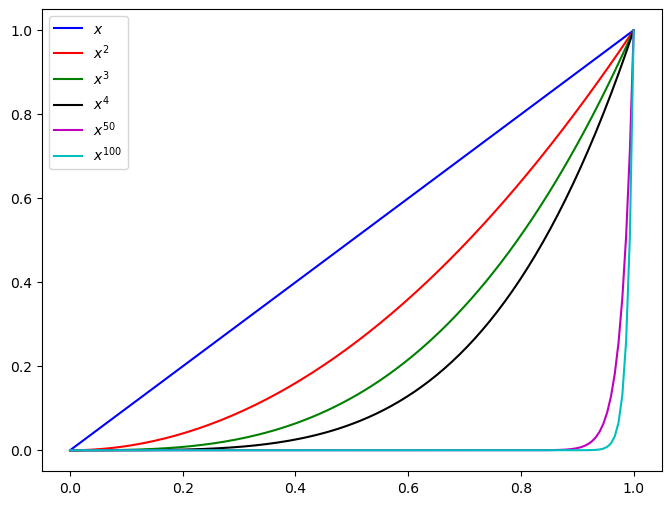
\includegraphics{"Temas/Tema 4/Gráfica 1.png"}
\end{figure}


\begin{itemize}[label=\color{red}\textbullet, leftmargin=*]
	\item \color{lightblue}Ejemplo
\end{itemize}
La sucesión $\left(\dfrac{x^n}{1+x^n}\right)_n$ converge puntualmente en el intervalo cerrado $[0,+\infty)$ a la función $f$ definida en tal intervalo por \[ f(x)=\left\{\begin{array}{ll}
	0 & \text{si }0\le x <1\\
	\frac{1}{2} & \text{si }x=1\\
	1 & \text{si } x >1\\
\end{array}\right.. \]

\begin{figure}[h]
	\centering
	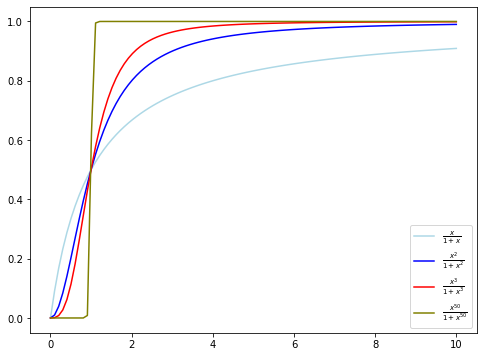
\includegraphics[width=0.7\textwidth]{"Temas/Tema 4/Gráfica 2.png"}
\end{figure}


La convergencia puntual puede expresarse en términos similares a los de la convergencia de sucesiones numéricas.
\begin{itemize}[label=\color{red}\textbullet, leftmargin=*]
	\item \color{lightblue}Definición (Otra forma para definir la convergencia puntual)
\end{itemize}
Sea $(f_n)$ una sucesión de funciones definidas en un conjunto $I,M$ un subconjunto de $I,f$ una función definida en $M$. La sucesión $(f_n)$ converge puntualmente a $f$ en $M$ si y sólo si para cada $x\in M$ y para cada $\epsilon>0$ existe un $N=N(\epsilon,x)$ tal que siempre que $n>N(\epsilon,x)$ se verifica $|f_n(x)-f(x)|<\epsilon$.

Análogo para la condición de Cauchy.
\begin{itemize}[label=\color{red}\textbullet, leftmargin=*]
	\item \color{lightblue}Definición
\end{itemize}
Una serie de funciones $\sum_{n=1}^{\infty}f_n$ es un par ordenado de sucesiones de funciones $\left((f_n),(s_n)\right)$ relacionadas por la condición de que para cada $n\in\mathbb{N}$ es \[ s_n=f_1+f_2+\cdots+f_n. \] Para cada $n\in\mathbb{N}$, el término $n$-ésimo de la primera sucesión, $f_n$, recibe el nombre de término $n$-ésimo de la serie; el término $n$-ésimo de la segunda sucesión, $s_n$, funciones converge puntualmente a una función $f$ en un conjunto $M$ si lo hace la sucesión de sus sumas parciales. En tal caso, la función $f$ es la suma de la serie en el conjunto $M$.
\begin{itemize}[label=\color{red}\textbullet, leftmargin=*]
	\item \color{lightblue}Ejemplo
\end{itemize}
La serie de funciones $\sum_{n=1}^{\infty}x^{n-1}$ converge puntualmente en $(-1,1)$ y su suma es la función $f(x)=\dfrac{1}{1-x}$, si $-1<x<1$.
\subsection{Convergencia uniforme}
El estudio de las sucesiones de funciones abre al menos dos interesantes opciones: de un lado, podemos construir nuevas funciones como límites de funciones conocidas; de otro, podemos pensar en sustituir, en ciertos problemas, una función dada por funciones que la aproximan y que pueden tener un comportamiento mejor controlado respecto a la situación que nos interese. En cualquiera de los dos casos, la primera tareas es examinar qué propiedades de las funciones que forman la sucesión se traspasan a la función límite.
\begin{itemize}[label=\color{red}\textbullet, leftmargin=*]
	\item \color{lightblue}Definición
\end{itemize}
Sea $(f_n)$ una sucesión de funciones definidas en un conjunto $I,M$ un subconjunto de $I, f$ una función definida en $M$. Se dice que la sucesión $(f_n)$ converge uniformemente a $f$ en $M$ si para cada $\epsilon>0$ existe un $N=N(\epsilon)$, para todo $x\in M$ se verifica $\left|f_n(x)-f(x)\right|<\epsilon$.

Es obvio que toda sucesión $(f_n)$ que converge uniformemente a una función $f$ en $M$, también converge puntualmente a $f$ en $M$.
\subsection{Series de potencias}
\begin{itemize}[label=\color{red}\textbullet, leftmargin=*]
	\item \color{lightblue}Definición
\end{itemize}
Sea $(a_n)_n$ y $x_0\in\mathbb{R}$, se llama serie de potencias de centro $x_0$ y coeficientes $a_n$ a la serie funcional $\sum_{n=1}^{\infty}a_n(x-x_0)^n$.

Obsérvese que el campo de convergencia no es vacío pues la serie converge en $x_0$.
\subsubsection{Convergencia uniforme de las series de potencias}
\begin{itemize}[label=\color{red}\textbullet, leftmargin=*]
	\item \color{lightblue}Teorema
\end{itemize}
Sea la serie de potencias $\sum_{n=1}^{\infty}a_n(x-x_0)^n$, si $\dfrac{1}{\lim_{n\to\infty}\sqrt[n]{|a_n|}}=r>0$, entonces se verifica: 
\begin{enumerate}[label=\arabic*)]
	\item Para cada $x\in(x_0-r,x_0+r)$, la serie $\sum_{n=1}^{\infty}a_n(x-x_0)^n$ es absolutamente convergente.
	\item Para cada $x\in\mathbb{R}\backslash\left[x_0-r,x_0+r\right]$, la serie $\sum a_n(x-x_0)^n$ no converge.
	\item Si $x$ es tal que $|x-x_0|=r$, no se puede asegurar nada.
\end{enumerate}
A $r=\dfrac{1}{\lim_{n\to\infty}\sqrt[n]{|a_n|}}$ se le llama \textcolor{lightblue}{radio de convergencia de la serie}. También se puede utilizar para su cálculo el límite. \[ r=\lim_{n\to\infty}\left|\dfrac{a_n}{a_{n+1}}\right|, \] que coincide con el valor anterior. A $(x_0-R,x_0+R)$ se le llama \textcolor{lightblue}{dominio de convergencia} de la serie. Evidentemente, las series $\sum_{n=0}^{\infty}a_nx^n$ y $\sum_{n=0}^{\infty}a_n(x-x_0)^n$ tienen el mismo radio de convergencia.
\begin{itemize}[label=\color{red}\textbullet, leftmargin=*]
	\item \color{lightblue}Teorema
\end{itemize}
Sea la serie de potencias $\sum_{n=0}^{\infty}a_n(x-x_0)^n$ y $r>0$ su radio de convergencia. Entonces $\forall[a,b]\subset(x_0-r,x_0+r)$, la serie $\sum_{n=0}^{\infty}a_n(x-x_0)^n$ es uniformemente convergente en $[a,b]$.
\begin{itemize}[label=\color{red}\textbullet, leftmargin=*]
	\item \color{lightblue}Teorema
\end{itemize}
Sea la serie de potencias $\sum_{n=0}^{\infty}a_n(x-x_0)^n$ y $r>0$ su radio de convergencia. Si además es convergente en $x=x_0+r$ (o en $x=x_0-r$), entonces la serie es uniformemente convergente en $[a,x_0+r]$ (respectivamente, en $[x_0-r,a]$) siendo $a\in(x_0-r,x_0+r)$.
